\documentclass[11pt,letterpaper,oneside]{book}
\usepackage{listings}
%\usepackage{color}
\usepackage[usenames,dvipsnames,svgnames,table]{xcolor}
\usepackage{graphicx}
%\usepackage{fancybox}
\usepackage{float}
\usepackage{hyperref}
\usepackage{pdflscape}
\usepackage{multicol}
\usepackage{caption}
\usepackage{courier}
\usepackage[letterpaper]{geometry}

%http://stackoverflow.com/questions/741985/latex-source-code-listing-like-in-professional-books
%\usepackage{caption}
%\DeclareCaptionFont{white}{\color{white}}
%\DeclareCaptionFormat{listing}{\colorbox{gray}{\parbox{\textwidth}{#1#2#3}}}
%\captionsetup[lstlisting]{format=listing,labelfont=white,textfont=white}

\hypersetup{colorlinks,%
citecolor=black,%
filecolor=black,%
linkcolor=black,%
urlcolor=black,%
}

\lstset{
basicstyle=\fontsize{10}{11}\ttfamily,
keywordstyle=\color{blue},
commentstyle=\color{DarkGreen},
stringstyle=\color{red},
numbers=left,
numberstyle=\tiny,
frame=tb,
%columns=fullflexible,
showstringspaces=false
captionpos=b,
numbersep=5pt,
breaklines=true,                        
breakatwhitespace=false 
}

\setcounter{secnumdepth}{4}

\title{OpenStack Havana}
\author{Joseph Callen}

\begin{document}
\frontmatter


\maketitle
\newenvironment{acknowledgements}%
    {\cleardoublepage\thispagestyle{empty}\null\vfill\begin{center}%
    \bfseries Acknowledgements\end{center}}%
    {\vfill\null}
        \begin{acknowledgements}
        I have read many articles from various sources I am sure I have missed to source them some along the way.  
        \end{acknowledgements}
\tableofcontents
\listoffigures
\listoftables
\lstlistoflistings
\mainmatter

%\renewcommand{\abstractname}{Executive Summary}
%\begin{abstract}
\chapter*{Executive Summary}
OpenStack can be difficult software package to install and configure for a novice.  I have created this document to guide someone through the install that I performed in the lab.  Hopefully with a "real world" example it should be easier to understand the various modules and concepts required for an OpenStack deployment.  This document was created with \LaTeX.
%\end{abstract}

\chapter{Introduction}
\section{Physical Hosts}
In order to test the installation and operational aspects of a true OpenStack environment I needed additional nodes.  Utilizing old laptop hardware I was able to create four additional virtual machines to run OpenStack services on.  The compute node remains physical.  I am still using the RDO Havana community edition on Fedora 19 x64.\\

\begin{table}[ht]
\caption{Physical Compute} % title of Table
\centering % used for centering table
\begin{tabular}{lccccc}
\hline 
\bf Hardware & • & \bf Dev & \bf Model & \bf Network & \bf Usage\\ \hline 
AMD Athlon Dual Core & 1 & eth0 & r8169 & Managment & Nova, Glance \&\\ 
8 GB RAM, 2 TB HD
& 2 & eth1 & e1000 & Instance uplink & Cinder\\ \hline

Levono T61 & 1 & eth0 & e1000e & Management \& & oVirt Node\\
Intel\textregistered Core2\texttrademark Duo CPU T7100, 4 GB RAM & & & & Instance Uplink  & \\ \hline

Dell Latitude D620 & 1 & eth0 & tg3 & Management \& & oVirt Node\\
Intel\textregistered Core2\texttrademark Duo CPU T5500, 4 GB RAM & & & & Instance Uplink & \\ \hline

Dell PE2850 & 1 & em1 & e1000 & Management & NFS\\
Intel\textregistered Xeon\texttrademark, 2 GB RAM, 3x146GB 10K & & & & Instance Uplink &\\ \hline
\end{tabular}
\end{table}


\section{oVirt}
oVirt is a management and host node virtualization package similar to vSphere.  It uses Linux KVM as the hypervisor with either Fedora or CentOS as the base OS.  The management console is web based.

\subsection{oVirt Engine Install}
Before installation DNS needs to be configured, including an A record of the oVirt engine and nodes.
%http://www.ovirt.org/Download
\begin{lstlisting}[caption={Install oVirt repo and package},language=bash]
yum localinstall http://ovirt.org/releases/ovirt-release-fedora.noarch.rpm
yum install -y ovirt-engine
engine-setup
\end{lstlisting}

\subsection{PXE}
To install an oVirt node the easiest method I have found is use PXE.  First lets convert the ISO to tftpboot. \textbf{Note:} This is an older release of ovirt-node, the current version has a bug with installation.\footnote{\href{https://bugzilla.redhat.com/show_bug.cgi?id=1032228}{Red Hat Bugzilla Bug \#1032228}}

\begin{lstlisting}[caption={Download and convert oVirt Node},language=bash]
wget http://resources.ovirt.org/releases/3.3/iso/ovirt-node-iso-3.0.1-1.0.2.vdsm.fc19.iso
livecd-iso-to-pxeboot ovirt-node-iso-3.0.1-1.0.2.vdsm.fc19.iso
\end{lstlisting}

\begin{lstlisting}[caption={Copy tftproot to root, restore SELinux context, change permissions},language=bash]
cp -R /tftpboot/ /
restorecon -Rv /tftpboot/
chmod -R 755 /tftpboot/
\end{lstlisting}

\begin{lstlisting}[caption={Enable TFTP},language=bash]
sed -i 's/disable.*=\ yes/disable\t\t\t= no/' /etc/xinetd.d/tftp
# or
vi /etc/xinetd.d/tftp
service tftp
{
        ...
        disable = no #change from yes to no
        ...
}
systemctl restart xinetd
\end{lstlisting}

\subsection{DHCP}
The DHCP server needs to be configured to provide addresses and PXE related configuration elements.
\begin{lstlisting}[caption={Install ISC DHCP server},language=bash]
yum install dhcp -y 
\end{lstlisting}

Below is a partial example of my DHCPd configuration file.  The most important section is "ovirt-server1". Options filename and next-server must be listed for PXE boot to function correctly.  The option filename will not change and should be listed as "pxelinux.0".
\begin{lstlisting}[caption={Example DHCPd configuration},language=bash]
authoritative;
ddns-update-style none;

ddns-domainname		"virtomation.com";
option domain-name 	"virtomation.com";
option domain-name-servers	10.53.252.123, 10.53.252.246;
option ntp-servers		10.53.252.123;
default-lease-time	86400;
option ip-forwarding	off;
...
subnet 10.53.253.0 netmask 255.255.255.0 {
	range 10.53.253.130 10.53.253.140;
	option routers 10.53.253.1;
	option subnet-mask	255.255.255.0;
}

# HOST - RHEV
host ovirt-server1  {
	hardware ethernet 00:15:C5:59:AE:36; # MAC from machine that will boot via PXE
	fixed-address 10.53.253.50; # Fixed IP address
	filename "pxelinux.0";
	next-server 10.53.252.50;  # DHCP Server
	option host-name "virkvmpaw001.virtomation.com";
}
...
\end{lstlisting}
After the configuration has been saved remember to restart dhcpd.
%\noindent\begin{minipage}{\linewidth}
\begin{lstlisting}[caption={Restart DHCPd},language=bash]
systemctl reload-or-try-restart dhcpd
\end{lstlisting}
%\end{minipage}
\subsection{oVirt Node Install}
The installation of the oVirt node is generally as easy as ESXi.  I am only displaying figures that need extra explanation.  Figure~\ref{fig:ovirt_04} shows the system volumes and sizes.  If you are using a USB flash drive set the log and swap to 5 MB.

\begin{figure}[ht]
	\caption{System Volumes}
	\centering
	\label{fig:ovirt_04}
	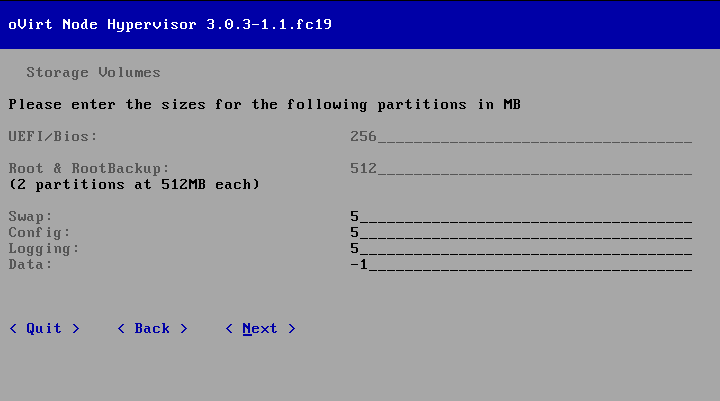
\includegraphics[scale=0.40]{./pictures/ovirt_006.png}
\end{figure}

The interfaces are not automatically configured.  Figure~\ref{fig:ovirt_07} shows the available interfaces, select an interface and hit enter.  In the next screen listed in Figure~\ref{fig:ovirt_08} configure the IP settings of the selected interface.

\begin{figure}[ht]
	\caption{Network Configuration}
	\centering
	\label{fig:ovirt_07}
	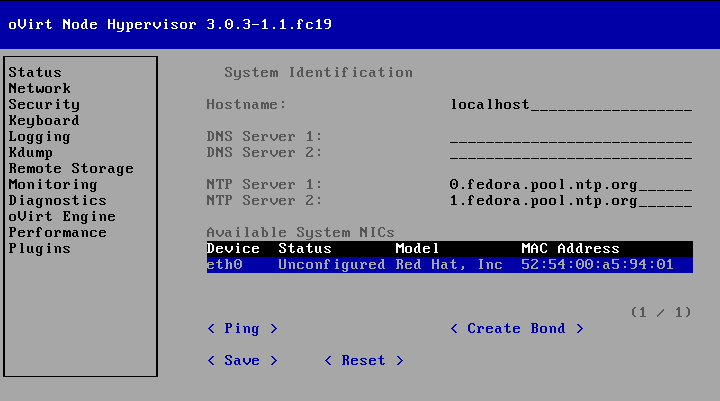
\includegraphics[scale=0.40]{./pictures/ovirt_009.png}
\end{figure}

\begin{figure}[ht]
	\caption{IP Configuration}
	\centering
	\label{fig:ovirt_08}
	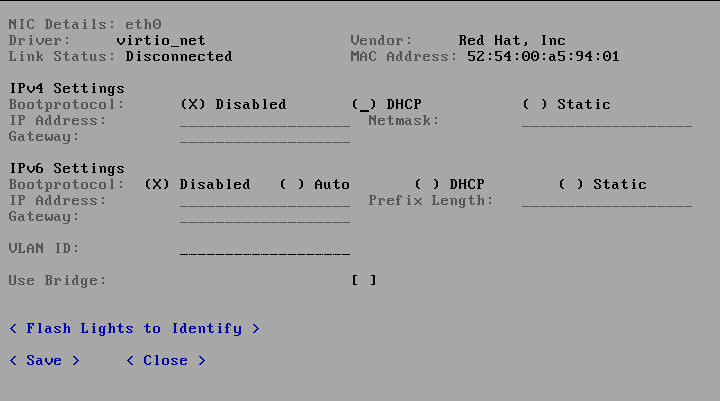
\includegraphics[scale=0.40]{./pictures/ovirt_010.png}
\end{figure}

Finally once the oVirt is available on the network you can configure it with the oVirt engine.  As displayed in Figure~\ref{fig:ovirt_10} configure the management server using either FQDN or IP and retrieve the certificate.  You can also set the optional password, which I recommend for a lab environment since it will also start ssh and set the root password.

\begin{figure}[ht]
	\caption{oVirt Engine Configuration}
	\centering
	\label{fig:ovirt_10}
	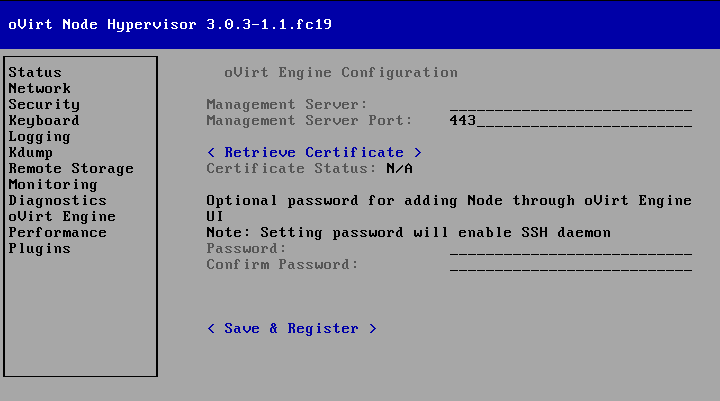
\includegraphics[scale=0.40]{./pictures/ovirt_011.png}
\end{figure}

\textbf{Note:} In my testing SELinux needed to be disabled before for any virtual machines would start.  To disable SELinux use the command listed below.  Unfortunately I haven't found a way to persist the changes after a reboot.  I would guess that re-mounting the filesystem read-write and changing setting in /etc/selinux/config file would work but I have yet to try it.

\begin{minipage}{\linewidth}
\begin{lstlisting}[caption={Disable SELinux},label={lst:disable_selinux},language=bash]
setenforce 0
\end{lstlisting}
\end{minipage}

\noindent Below is a screenshot of the oVirt Administration UI with the available hosts listed.
\begin{figure}[ht]
	\caption{Hosts in oVirt Engine }
	\centering
	\label{fig:ovirt_engine_01}
	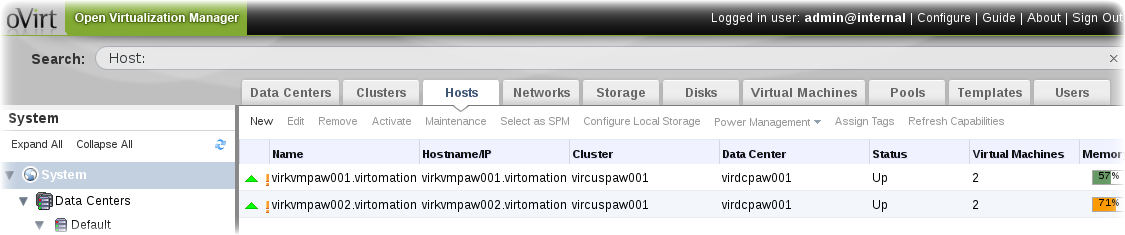
\includegraphics[scale=0.40]{./pictures/ovirt_engine_001.png}
\end{figure}

\chapter{All-In-One install with Neutron using VLANs}
\begin{figure}
	\caption{Compute Node}
	\centering
	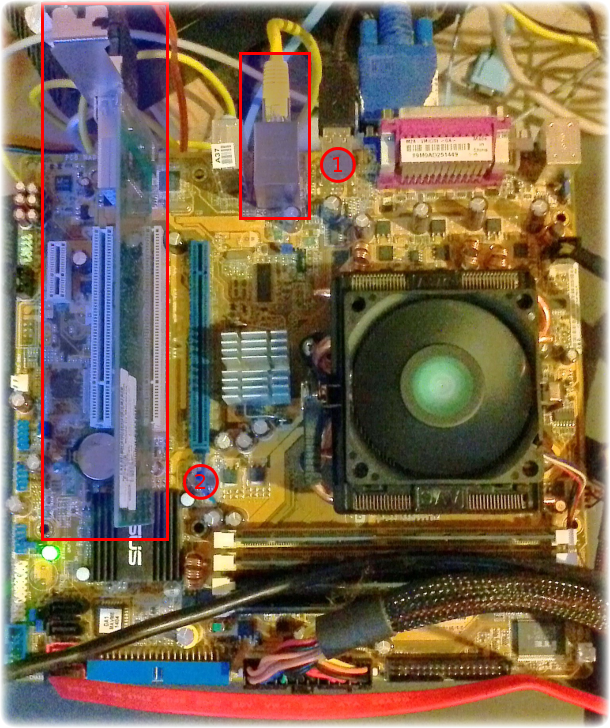
\includegraphics[scale=0.25]{./pictures/motherboard.png}
\end{figure}
\section{Physical Networking}

I have three VLAN 98 --- 100 configured on a dot1q trunk to interface p9p1 on a Fedora 19 host.  VLAN 100 has a gateway IP configured (10.53.100.1) on the Cisco Catalyst 4006.  VLAN 98 and 99 are non-routed vlans, at least as configured on the catalyst, so they have no gateway IP addresses configured, that will be provided by the neutron router.

\begin{figure}
	\caption{Cisco Catayst 4006}
	\centering
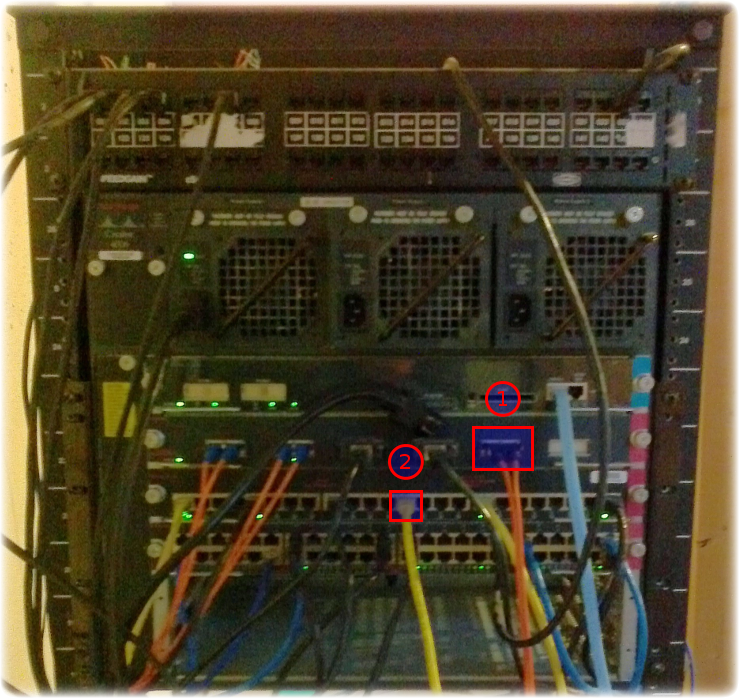
\includegraphics[scale=.35]{./pictures/c4006.png} 
\end{figure}

\begin{lstlisting}[caption={VLAN Configuration},language=bash]
interface Vlan98 
 no ip address 
end 
interface Vlan99 
 no ip address 
end 
interface Vlan100 
 ip address 10.53.100.1 255.255.255.0 
 ip helper-address 10.53.252.50 
end 
\end{lstlisting}

\begin{lstlisting}[caption={Instance uplink interface; gi2/5; \#1},language=bash]
interface GigabitEthernet2/5 
 switchport trunk encapsulation dot1q 
 switchport trunk allowed vlan 2-4,12,98-100,250-253 
 switchport mode trunk 
end 
\end{lstlisting}

\begin{lstlisting}[caption={Management interface; gi3/13; \#2},language=bash]
WS-C4006-SUPV#sh run int gi3/13 
Building configuration... 

Current configuration : 65 bytes 
! 
interface GigabitEthernet3/13 
 switchport access vlan 253 
end 
\end{lstlisting}


\section{Installation}

\subsection{Packstack}
\begin{lstlisting}[caption={Configure Packstack},language=bash]
DATE=`date +"%Y_%m_%d_%H_%M_%S"`
packstack --gen-answer-file=packstack-${DATE}
vi packstack-${DATE}
\end{lstlisting}
\begin{lstlisting}[caption={Answer file changes},language=bash]
CONFIG_NEUTRON_INSTALL=y
CONFIG_CINDER_VOLUMES_CREATE=n
CONFIG_NEUTRON_L3_EXT_BRIDGE=provider 
CONFIG_NEUTRON_OVS_TENANT_NETWORK_TYPE=vlan 
CONFIG_NEUTRON_OVS_VLAN_RANGES=inter-vlan:98:99
CONFIG_NEUTRON_OVS_BRIDGE_MAPPINGS=inter-vlan:br-inst 
CONFIG_NEUTRON_OVS_BRIDGE_IFACES=br-inst:p9p1 
\end{lstlisting}

\begin{lstlisting}[caption={Execute Packstack},language=bash]
packstack --answer-file=packstack-${DATE}
\end{lstlisting}
\textbf{Note:} Monitor the progress in detail via /var/tmp/packstack/

\section{Neutron Networking}

\subsection{External}
Now we will configure VLAN 100 to be our external network.  First we need to source the keystone file created by packstack. % maybe see appendix

\begin{lstlisting}[caption={Create network},language=bash]
neutron net-create ext_vlan100 --provider:network_type vlan --provider:physical_network inter-vlan --provider:segmentation_id 100 --router:external=True
\end{lstlisting}

Create a subnet for ext\_vlan100, this will be used for floating addresses.

\begin{lstlisting}[caption={Create subnet},language=bash]
neutron subnet-create ext_vlan100 --gateway 10.53.100.1 --name ext_vlan100_subnet 10.53.100.0/24 --allocation-pool start=10.53.100.10,end=10.53.100.253 --enable_dhcp=False
\end{lstlisting}

\begin{lstlisting}[caption={Create router},language=bash]
neutron router-create ext_vlan100_router 
\end{lstlisting}

\begin{lstlisting}[caption={Set gateway},language=bash]
neutron router-gateway-set ext_vlan100_router ext_vlan100
\end{lstlisting}

\subsection{Tenant}
\begin{lstlisting}[caption={Create network},language=bash]
TENANT_ID=$(keystone tenant-list|awk '/admin/ {print $2}') 
neutron net-create --tenant-id ${TENANT_ID} net01
\end{lstlisting}

\begin{lstlisting}[caption={Create subnet},language=bash]
neutron subnet-create net01 --name net01_subnet 192.168.98.0/24 
\end{lstlisting}
\begin{lstlisting}[caption={Add interface},language=bash]
neutron router-interface-add ext_vlan100_router net01_subnet 
\end{lstlisting}

The ext\_vlan\_router than becomes the default gateway for the vlan with an IP of 192.168.98.1. And the result as displayed in Horizon.

\subsection{Troubleshooting}

\begin{figure}
	\caption{VLAN Scenario}
	\centering
	\label{vlan}
	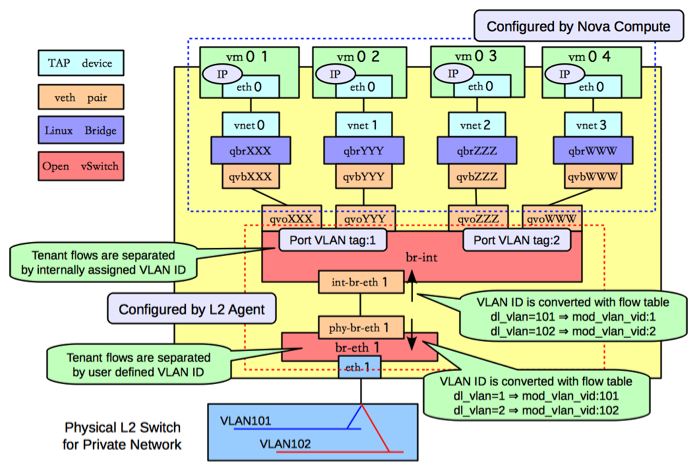
\includegraphics[scale=0.5]{./pictures/under-the-hood-scenario-2-ovs-compute.png}
\end{figure}

I believe OpenStack networking with Neutron is the most difficult part of the stack to understand.  The problem being just to have isolated tenant networks requires linux bridge, open vswitch bridge, and virtual Ethernet devices.  I have created a python script to better understand the relationship between a virtual machine and those devices.

The table below shows the interfaces between the vm and int-br-eth (as shown in Figure~\ref{vlan}), where a majority of the devices are configured.

\lstinputlisting[caption={map\_router.py script},language=Python]{map_router.py}

\begin{lstlisting}[caption={map\_router output},language=bash]
Troubleshooting commands:
ip netns exec qrouter-2672c623-3b4e-4c28-9f4f-505b17a25542 ip a
ip netns exec qrouter-2672c623-3b4e-4c28-9f4f-505b17a25542 ip r
ip netns exec qrouter-2672c623-3b4e-4c28-9f4f-505b17a25542 iptables -t nat -L -nv
ip netns exec qrouter-2672c623-3b4e-4c28-9f4f-505b17a25542 iptables -S -t nat
ip netns exec qrouter-2672c623-3b4e-4c28-9f4f-505b17a25542 ping 8.8.8.8
+----------------+--------------------------------------+
| Property       | Value                                |
+----------------+--------------------------------------+
| OpenStack Name | ubuntu1204                           |
| QEMU Name      | instance-00000016                    |
| UUID           | e2c0d2b3-05c6-45e9-ad52-6f11647badbb |
| tap            | tap0598ef4e-cd                       |
| linuxbridge    | qbr0598ef4e-cd                       |
| MAC Address    | fa:16:3e:65:a7:1f                    |
| VETH Pair #1   | qvb0598ef4e-cd                       |
| VETH Pair #2   | qvo0598ef4e-cd                       |
| ovsbridge      | br-int                               |
| TAG            | 2                                    |
| VLAN           | 98                                   |
+----------------+--------------------------------------+
\end{lstlisting}
\chapter{Multinode install using Neutron with GRE}

\section{Physical Networking}
The configuration of the physical network is significantly reduced when using tunneling.  To make configuration easier I only used VLAN 253.

\begin{lstlisting}[caption={Nova Node uplink interface; gi2/5},language=bash]
interface GigabitEthernet2/5
 switchport access vlan 253
 switchport mode access
!
\end{lstlisting}
\begin{lstlisting}[caption={Virtual Machine uplink; gi3/4},language=bash]
interface GigabitEthernet3/4
 switchport access vlan 253
 switchport mode access
!
\end{lstlisting}

\begin{lstlisting}[caption={Virtual Machine uplink; gi3/20},language=bash]
interface GigabitEthernet3/20
 switchport access vlan 253
 switchport mode access
!
\end{lstlisting}

\section{Installation}

First things first, we need to completely remove the OpenStack install on the physical compute node.  To accomplish that I used the big hammer method.\footnote{\href{http://openstack.redhat.com/Uninstalling_RDO}{Uninstalling RDO}}  This would also be useful if Packstack has issues with installation and you would like to start over without removing a snapshot or redeploying.

\begin{lstlisting}[caption={Remove OpenStack from all nodes},language=bash]
ssh root@viropspaw002 'bash -s' < big_hammer.sh
for i in {1..3}; do ssh root@viropspaw01$i 'bash -s' < big_hammer.sh; done
\end{lstlisting}


\subsection{DNS}
My current DNS servers are Windows 2012.  To add multiple entries its just easier to use PowerShell, which is listed below.

\begin{lstlisting}[caption={DNS Entries},language=bash]
Add-DnsServerResourceRecordA -Name "viropspaw002" -ZoneName "virtomation.com" -IPv4Address 10.53.253.70 -ComputerName 10.53.252.123
Add-DnsServerResourceRecordA -Name "viropspaw010" -ZoneName "virtomation.com" -IPv4Address 10.53.253.90 -ComputerName 10.53.252.123
Add-DnsServerResourceRecordA -Name "viropspaw011" -ZoneName "virtomation.com" -IPv4Address 10.53.253.100 -ComputerName 10.53.252.123
Add-DnsServerResourceRecordA -Name "viropspaw012" -ZoneName "virtomation.com" -IPv4Address 10.53.253.110 -ComputerName 10.53.252.123
Add-DnsServerResourceRecordA -Name "viropspaw013" -ZoneName "virtomation.com" -IPv4Address 10.53.253.120 -ComputerName 10.53.252.123
\end{lstlisting}

\subsection{Virtual Machine Deployment}
Just like with vSphere we will create a template to use for virtual machine deployment.  First we need to upload the Fedora 19 x64 iso to the NFS domain. 

\begin{lstlisting}[caption={Upload ISO},language=bash]
wget http://download.fedoraproject.org/pub/fedora/linux/releases/19/Fedora/x86_64/iso/Fedora-19-x86_64-netinst.iso
ovirt-iso-uploader -i ISO_NFS upload Fedora-19-x86_64-netinst.iso
\end{lstlisting}

\subsubsection{Disable firewalld} 
We need to disable firewalld and replace it with iptables as it is not supported with Havana.\footnote{\href{https://bugzilla.redhat.com/show_bug.cgi?id=981583}{Red Hat Bugzilla Bug \#981583}}
\begin{lstlisting}[caption={Disable firewalld, install iptables},language=bash]
yum install iptables -y
systemctl disable firewalld 
systemctl enable iptables 
\end{lstlisting}
\subsubsection{Disable SELinux}  
The issue with SELinux and OpenStack has been resolved\footnote{\href{https://bugzilla.redhat.com/show_bug.cgi?id=995780}{Red Hat Bugzilla Bug \#995780}}, lets disable it anyway.
\begin{lstlisting}[caption={Disable SELinux},language=bash]
setenforce 0 # does not persist 
sed -i 's/SELINUX=enforcing/SELINUX=disabled/' /etc/selinux/config
# or
vi /etc/selinux/config
...
SELINUX=disabled
...
\end{lstlisting}

\subsection{SSH Keys}
\begin{lstlisting}[caption={SSH Key Copy},language=bash]
echo "StrictHostKeyChecking no" >> /root/.ssh/config
for i in {1..3}
do
	ssh-copy-id -i /root/.ssh/id_rsa.pub viropspaw01$i
done
ssh-copy-id -i /root/.ssh/id_rsa.pub viropspaw002
\end{lstlisting}

\subsection{Packstack}
\begin{lstlisting}[caption={Packstack remote install after big hammer},language=bash]
for i in {0..3}; do ssh viropspaw01$i "yum install openstack-packstack -y"; done
\end{lstlisting}

\begin{lstlisting}[caption={Configure Packstack},language=bash]
DATE=`date +"%Y_%m_%d_%H_%M_%S"`
packstack --gen-answer-file=packstack-${DATE}
vi packstack-${DATE}

\end{lstlisting}

Listing~\ref{lst:packstack_gre} is the differences between a newly generated answer file and one that has been configured for GRE.  The left side is the original and the right has the changes.  Occasionally when the line is too long the change is forced to a new line.

%\newgeometry{top=.25in}
%\clearpage
%\begin{landscape}
\begin{lstlisting}[caption={Changes in Packstack answer file},label={lst:packstack_gre},language=bash,breakatwhitespace=true]
CONFIG_CEILOMETER_INSTALL=n
CONFIG_NTP_SERVERS=10.53.252.123,10.53.252.246
CONFIG_NAGIOS_INSTALL=y
CONFIG_GLANCE_HOST=10.53.253.70
CONFIG_CINDER_HOST=10.53.253.70
CONFIG_CINDER_VOLUMES_CREATE=n
CONFIG_NOVA_COMPUTE_HOSTS=10.53.253.70
CONFIG_NEUTRON_SERVER_HOST=10.53.253.100
CONFIG_NEUTRON_L3_HOSTS=10.53.253.100
CONFIG_NEUTRON_DHCP_HOSTS=10.53.253.100
CONFIG_NEUTRON_METADATA_HOSTS=10.53.253.100
CONFIG_NEUTRON_OVS_TENANT_NETWORK_TYPE=gre
CONFIG_NEUTRON_OVS_TUNNEL_RANGES=1:1000
CONFIG_NEUTRON_OVS_TUNNEL_IF=eth1
CONFIG_HORIZON_HOST=10.53.253.120
CONFIG_NAGIOS_HOST=10.53.253.120
\end{lstlisting}
%\restoregeometry
%\end{landscape}

\begin{lstlisting}[caption={Execute Packstack},language=bash]
packstack --answer-file=packstack-${DATE}
\end{lstlisting}
\textbf{Note:} Monitor the progress in detail via /var/tmp/packstack/

\section{Neutron Networking}
\begin{figure}[H]
	\caption{OpenStack Node Details}
	\centering
	\label{fig:openstack_neutron_gre}
	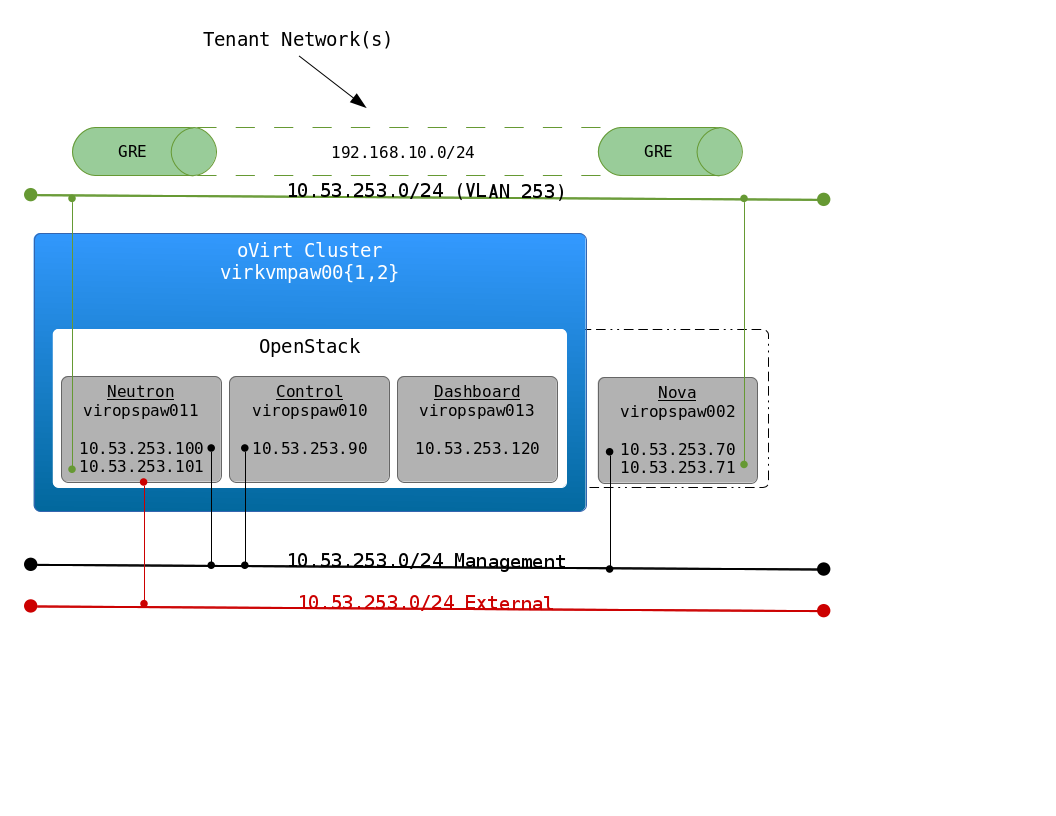
\includegraphics[scale=0.75]{./pictures/openstack_neutron_gre.png}
\end{figure}
%\newgeometry{top=.25in}
%\clearpage
%\begin{landscape}
%\begin{minipage}[b]{0.45\linewidth}
\begin{lstlisting}[caption={Nova Node Open vSwtich},language=bash]
ovs-vsctl show
95dc7e47-0b2b-49e9-82ae-da4b60dccb68
    Bridge br-tun
        Port br-tun
            Interface br-tun
                type: internal
        Port "gre-1"
            Interface "gre-1"
                type: gre
                options: {in_key=flow, local_ip="10.53.253.71", out_key=flow, remote_ip="10.53.253.101"}
        Port patch-int
            Interface patch-int
                type: patch
                options: {peer=patch-tun}
    Bridge br-int
        Port patch-tun
            Interface patch-tun
                type: patch
                options: {peer=patch-int}
        Port "qvo7ac76cfd-c8"
            tag: 4
            Interface "qvo7ac76cfd-c8"
        Port "qvoec307994-cd"
            tag: 4
            Interface "qvoec307994-cd"
        Port br-int
            Interface br-int
                type: internal
    ovs_version: "1.11.0"
\end{lstlisting}
%\end{minipage}
%\hspace{0.5cm}
%\begin{minipage}[b]{0.45\linewidth}
\begin{lstlisting}[caption={Neutron Node Open vSwtich},language=bash]
9a0a47e6-e002-4494-b217-5143e9419870
    Bridge br-int
        Port "tap5555b73f-79"
            tag: 1
            Interface "tap5555b73f-79"
                type: internal
        Port "qr-25c4c000-4b"
            tag: 1
            Interface "qr-25c4c000-4b"
                type: internal
        Port br-int
            Interface br-int
                type: internal
        Port patch-tun
            Interface patch-tun
                type: patch
                options: {peer=patch-int}
    Bridge br-tun
        Port patch-int
            Interface patch-int
                type: patch
                options: {peer=patch-tun}
        Port br-tun
            Interface br-tun
                type: internal
        Port "gre-2"
            Interface "gre-2"
                type: gre
                options: {in_key=flow, local_ip="10.53.253.101", out_key=flow, remote_ip="10.53.253.71"}
    Bridge br-ex
        Port "qg-f7e557b2-b4"
            Interface "qg-f7e557b2-b4"
                type: internal
        Port "eth2"
            Interface "eth2"
        Port br-ex
            Interface br-ex
                type: internal
    ovs_version: "1.11.0"
\end{lstlisting}
%\end{minipage}
%\restoregeometry
%\end{landscape}


\subsection{External}
\begin{lstlisting}[caption={Create public network and subnet},language=bash]
neutron net-create public_network --router:external=True
neutron subnet-create public_network 10.53.253.0/24 --name public_subnet --enable_dhcp=False --allocation-pool start=10.53.253.150,end=10.53.253.160 --gateway=10.53.253.1
\end{lstlisting}

\subsection{Tenant}
\begin{lstlisting}[caption={Create admin tenant router, network and subnet},language=bash]
neutron router-create admin_router
neutron net-create admin_network
neutron subnet-create admin_network 192.168.10.0/24 --name admin_subnet
\end{lstlisting}

\begin{lstlisting}[caption={Set the router gateway},language=bash]
neutron router-gateway-set admin_router public_network
\end{lstlisting}




\subsection{Troubleshooting}
This section is devoted to resolving issues that I encountered while installing and configuring OpenStack.
\subsubsection{Issue deleting floating IP port}
\begin{lstlisting}[caption={Stop Neutron Services},language=bash]
NEUTRON_SERVICES=`systemctl --all --full --no-page -t service  | grep neutron | awk '{print $1}'`
for SERVICE in $NEUTRON_SERVICES; do systemctl stop $SERVICE; done
\end{lstlisting}

\begin{lstlisting}[caption={Find the MariaDB root password},language=bash]
grep -i mysql packstack-2013_12_05_10_01_35 
...
# Username for the MySQL admin user
CONFIG_MYSQL_USER=root
# Password for the MySQL admin user
CONFIG_MYSQL_PW=5729f733fd9f4731
...
\end{lstlisting}
\begin{lstlisting}[caption={Login to MariaDB},language=bash]
mysql -u root -p
\end{lstlisting}
\begin{lstlisting}[caption={Get the ID for the floating IP and delete},language=sql]
use ovs_neutron;
select * from floatingips;
+--------------------------------------+
| id                                   |
+--------------------------------------+
| f5af35d0-7a4c-459c-85dc-9f6af9fb1b6c |
+--------------------------------------+
delete from floatingips where id = 'f5af35d0-7a4c-459c-85dc-9f6af9fb1b6c'
\end{lstlisting}

\section{OpenDaylight}
I just started to test with OpenDaylight controller.  I am fairly certain that I set this up incorrectly.  The only positive is a web-based UI for viewing Open vSwitch / OpenStack networking.

\begin{figure}[H]
	\caption{OpenDaylight Controller UI}
	\centering
	\label{fig:opendaylight_ctrl_ui}
	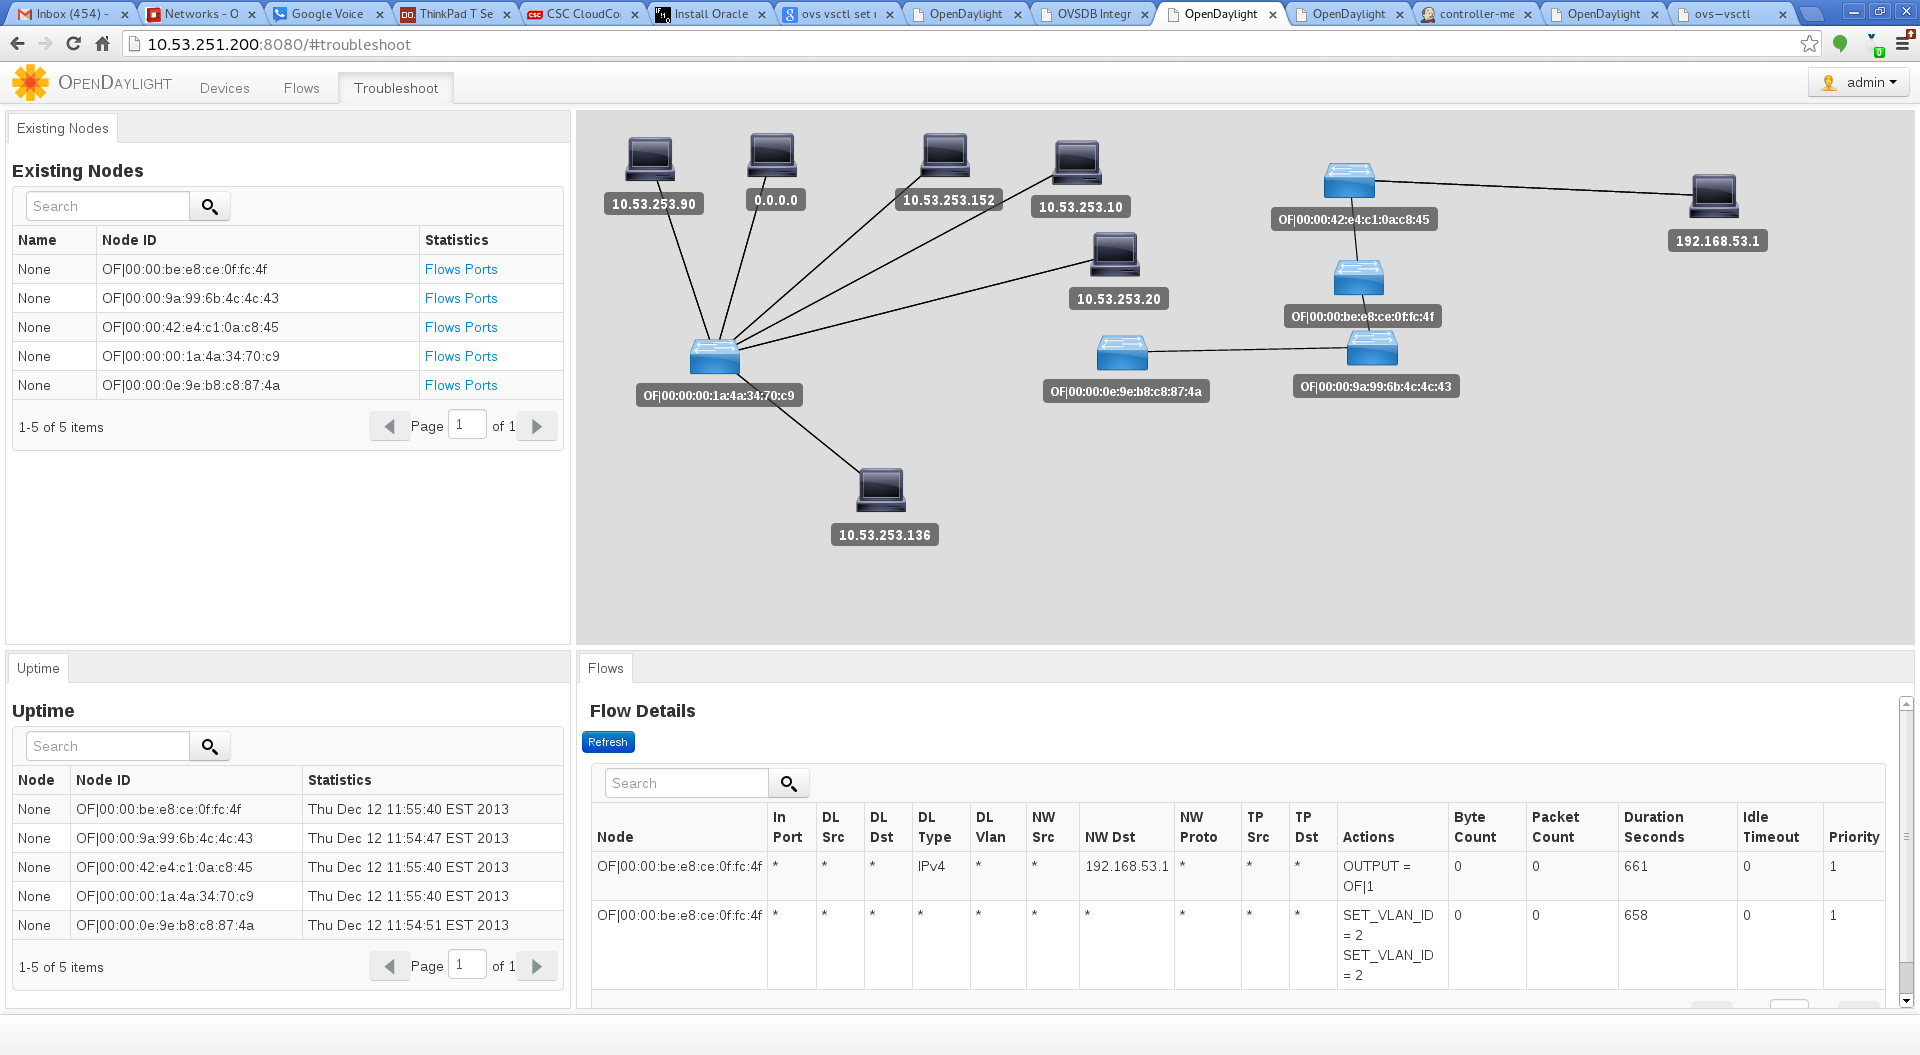
\includegraphics[scale=0.25]{./pictures/OpenDaylightController.png}
\end{figure}

%https://wiki.opendaylight.org/view/OpenDaylight_Controller:Installation

\subsection{Install Controller}
I built a new Fedora 19 x64 virtual machine for the OpenDaylight controller.   


\begin{lstlisting}[caption={Install Oracle Java JDK},language=bash]
sudo yum install jdk-7u45-linux-x64.rpm
\end{lstlisting}
\begin{lstlisting}[caption={Disable firewalld},language=bash]
systemctl stop firewalld
systemctl disable firewalld
\end{lstlisting}
\begin{lstlisting}[caption={Get the latest controller},language=bash]
wget https://jenkins.opendaylight.org/controller/job/controller-merge/lastSuccessfulBuild/artifact/opendaylight/distribution/opendaylight/target/distribution.opendaylight-osgipackage.zip
unzip distribution.opendaylight-osgipackage.zip
\end{lstlisting}
\begin{lstlisting}[caption={Start the controller},language=bash]
cd opendaylight
./run.sh
\end{lstlisting}

\subsection{Configure Open vSwitch}

\begin{lstlisting}[caption={Neutron node set controller and manager},language=bash]
ovs-vsctl set-controller br-tun tcp:10.53.251.200
ovs-vsctl set-controller br-ex tcp:10.53.251.200
ovs-vsctl set-controller br-int tcp:10.53.251.200
ovs-vsctl set-manager tcp:10.53.251.200
\end{lstlisting}

\begin{lstlisting}[caption={Nova node set controller},language=bash]
ovs-vsctl set-controller br-tun tcp:10.53.251.200
ovs-vsctl set-controller br-int tcp:10.53.251.200
\end{lstlisting}


\chapter{Instances}
\section{Security Group Configuration}
RDO/Packstack creates two "default" security groups.  This seems to cause issues with iptables as the instances created are not network available.  First we will delete the rules.

\begin{lstlisting}[caption={Delete existing security group rules},language=bash]
SECURITY_GROUP_RULE_LIST=`neutron security-group-rule-list \
--column id --format csv \
| awk 'NR > 1 split($0, a, "\"") {print a[2]}'`
for ID in ${SECURITY_GROUP_RULE_LIST}; 
do 
neutron security-group-rule-delete $ID; 
done
\end{lstlisting}

Now we will delete the groups themselves.  If there is a error stating that the group cannot be deleted because a rule exists that is OK.  Just as long as one of the "default" groups has been deleted.
\begin{lstlisting}[caption={Delete existing security groups},language=bash]
SECURITY_GROUP_LIST=`neutron security-group-list --column id --format csv | awk 'NR > 1 split($0, a, "\"") {print a[2]}'`
for ID in ${SECURITY_GROUP_LIST}; 
do 
neutron security-group-delete $ID; 
done
\end{lstlisting}

The rules have been deleted lets create our own.  Of course these rules open all available ports, probably not what you want to do in production.  
\begin{lstlisting}[caption={},language=bash]
neutron security-group-rule-create --protocol icmp --direction ingress default 
neutron security-group-rule-create --protocol tcp --port-range-min 1 --port-range-max 65535 --direction ingress default 
neutron security-group-rule-create --protocol tcp --port-range-min 1 --port-range-max 65535 --direction egress default 
\end{lstlisting}
\section{Create Images}
OpenStack documentation has details for obtaining images for QEMU/KVM Windows and Linux flavors with cloud-init already installed. See link in sources.
\subsection{Ubuntu LTS 12.04}
\subsection{Windows 2012 R2}
The problem that I ran into was that my / was too small. When using LVM for KVM machines qcow2
images must be converted to raw and copied (dd) into the volume that is created. Glance and/or Cinder
use the / filesystem to perform this action (I need to research more information about this). So in order
to add Windows I had to manually convert qcow2 image to RAW within a temporary logical volume
and then copy into a new logical volume.
\begin{lstlisting}[caption={Windows 2012 R2 Image Create},language=bash]
gunzip -cd windows_server_2012_r2_standard_eval_kvm_20131031.qcow2.gz | glance image-create --name "Windows Server 2012 R2 Std Eval" --disk-format=qcow2 --container-format=bare 
+------------------+--------------------------------------+ 
| Property         | Value                                | 
+------------------+--------------------------------------+ 
| checksum         | 5fb0a80e56479d31f8b5c1a8e6339206     | 
| container_format | bare                                 | 
| created_at       | 2013-11-06T17:35:34                  | 
| deleted          | False                                | 
| deleted_at       | None                                 | 
| disk_format      | qcow2                                | 
| id               | 32c94fcb-ea3a-4c69-8a49-a6095b8b25ba | 
| is_public        | False                                | 
| min_disk         | 0                                    | 
| min_ram          | 0                                    | 
| name             | Windows Server 2012 R2 Std Eval      | 
| owner            | c70e8967165a4b57b8cd0d4265104f01     | 
| protected        | False                                | 
| size             | 17182752768                          | 
| status           | active                               | 
| updated_at       | 2013-11-06T17:39:48                  | 
+------------------+--------------------------------------+ 

lvcreate -n temp -L 100G cinder-volumes
mkfs.ext3 /dev/cinder-volumes/temp
mount /dev/cinder-volumes/temp /mnt/tmp/ 
cd /mnt/tmp/ 
qemu-img convert /var/lib/glance/images/32c94fcb-ea3a-4c69-8a49-a6095b8b25ba -O raw ./windows.raw
\end{lstlisting}
\section{Create Instance}
Before we create an instance lets import the public key.
\begin{lstlisting}[caption={Add public key},language=bash]
nova keypair-add userkey --pub-key /root/.ssh/id_rsa.pub
\end{lstlisting}
When working with a Windows OS the Administrator password will be set by nova.  To retrieve the password use the following command. 
\begin{lstlisting}[caption={Windows administrator password},language=bash]
nova get-password windows /root/.ssh/id_rsa 
38MQ21a1LxYMpH
\end{lstlisting}
\appendix
\chapter{Notes}
\section{Neutron}
With external egress and ingress virtual machine traffic traversing the Neutron node it should be highly-available.  How is this accomplished?  What is the length of downtime or in a GRE/VXLAN scenario have multiple "uplinks" to another Neutron host? 
\begin{lstlisting}[language=bash]
Port "gre-1"
            Interface "gre-1"
                type: gre
                options: {in_key=flow, local_ip="10.53.253.71", out_key=flow, remote_ip="10.53.253.101"}
\end{lstlisting}
\section{Horizon}
How to limit users on Horizon to create instances with new volume.
\section{Cinder}
When deleting a volume cinder by default will dd /dev/zero – this takes forever.
\begin{lstlisting}[caption={Change Cinder volume clear},language=bash]
sed -i 's/#volume_clear=zero/volume_clear=none/' /etc/cinder/cinder.conf
# or
vi /etc/cinder/cinder.conf
...
# Method used to wipe old voumes (valid options are: none, 
# zero, shred) (string value) 
volume_clear=none
...
SERVICES=`systemctl --no-page --full -t service | grep openstack-cinder | awk '{print $1}'` 
for CINDER in $SERVICES; do systemctl restart $CINDER; done
\end{lstlisting}
\section{Nova}
How to properly configure Windows images with the correct QEMU/KVM settings?
\chapter{Links}
\href{http://docs.openstack.org/grizzly/openstack-network/admin/content//under_the_hood_openvswitch.html}{Under the hood Open vSwitch}\\
\href{http://openstack.redhat.com/Neutron\_with\_OVS\_and\_VLANs}{Neutron with OVS and VLANs}\\
\href{http://www.blog.sandro-mathys.ch/2013/08/install-rdo-havana-2-on-fedora-19-and.html}{Install RDO Havana on Fedora 19}\\
\href{http://docs.openstack.org/image-guide/content/ch\_obtaining\_images.html}{Obtaining Images for OpenStack}\\
\href{http://www.markhneedham.com/blog/2013/06/26/unixawk-extracting-substring-using-a-regular-expression-with-capture-groups/}{Awk extracting substring using regular expressions with capture groups}\\

\end{document}